
\documentclass[tikz,border=2]{standalone}
\usetikzlibrary{shadows,arrows,shapes,positioning,calc,backgrounds,fit}
\usepackage{amssymb}
\usepackage{array}
\usepackage{colortbl}
\pdfpageattr {/Group << /S /Transparency /I true /CS /DeviceRGB>>}
\newcommand{\lens}[7]{ % ux,uy,vx,vy,in,out,color
\path[fill=#7,out=#5,in=#6] (#1,#2) -- (#3,#4);
}
\newcommand{\lensarrow}[7]{ % ux,uy,vx,vy,in,out,arrowwidth
\draw[-{Latex[width=#7},out=#5,in=#6] (#1,#2) -- (#3,#4);
}

% custom colors
\definecolor{myBlue}{HTML}{0060AD}
\definecolor{myRed}{HTML}{DD181F}

\begin{document}
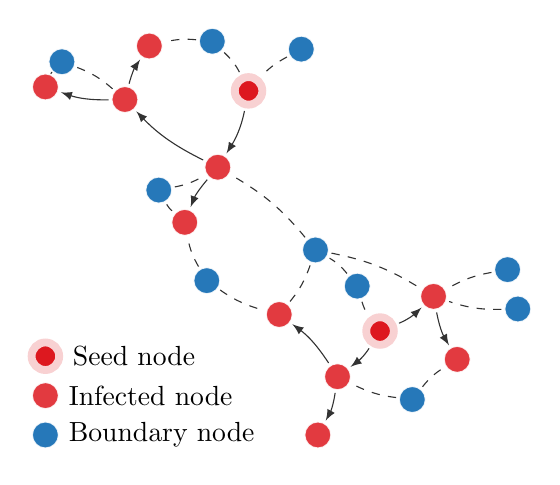
\begin{tikzpicture}
[
arr/.style={>=latex, shorten >=1pt, shorten <=1pt},
source/.style={circle,minimum width=3.5mm,fill=myRed,draw=myRed!20,line width=1mm},
infected/.style={circle,minimum width=2.5mm,fill=myRed,draw=white,opacity=0.850000},
boundary/.style={circle,minimum width=2.5mm,fill=myBlue,draw=white,opacity=0.850000},
]

% Nodes
\node[draw,source] (1) at (4.25,1.32) {};
\node[draw,infected] (2) at (4.93,1.76) {};
\node[draw,infected] (3) at (3.71,0.74) {};
\node[draw,infected] (4) at (5.23,0.96) {};
\node[draw,infected] (5) at (2.97,1.53) {};
\node[draw,infected] (6) at (3.46,0.0) {};
\node[draw,source] (7) at (2.58,4.37) {};
\node[draw,infected] (8) at (2.19,3.4) {};
\node[draw,infected] (9) at (1.01,4.26) {};
\node[draw,infected] (10) at (1.77,2.7) {};
\node[draw,infected] (11) at (1.32,4.94) {};
\node[draw,infected] (12) at (0.0,4.42) {};
\node[draw,boundary] (13) at (3.43,2.35) {};
\node[draw,boundary] (14) at (4.66,0.45) {};
\node[draw,boundary] (15) at (0.21,4.74) {};
\node[draw,boundary] (16) at (2.12,5.0) {};
\node[draw,boundary] (17) at (3.96,1.89) {};
\node[draw,boundary] (18) at (2.05,1.96) {};
\node[draw,boundary] (19) at (6.0,1.6) {};
\node[draw,boundary] (20) at (5.87,2.1) {};
\node[draw,boundary] (21) at (1.44,3.11) {};
\node[draw,boundary] (22) at (3.25,4.9) {};

% Edges
\draw[] (1) edge[,black!80,arr,,out=22.909999999999997,in=-137.09,->] (2);
\draw[] (1) edge[,black!80,arr,,out=-122.94999999999999,in=37.05,->] (3);
\draw[] (2) edge[,black!80,arr,,out=-79.44,in=120.56,->] (4);
\draw[] (3) edge[,black!80,arr,,out=123.13,in=-36.87,->] (5);
\draw[] (3) edge[,black!80,arr,,out=-98.67,in=61.33,->] (6);
\draw[] (7) edge[,black!80,arr,,out=-101.9,in=58.099999999999994,->] (8);
\draw[] (8) edge[,black!80,arr,,out=153.91,in=-46.09,->] (9);
\draw[] (8) edge[,black!80,arr,,out=-130.95999999999998,in=69.03999999999999,->] (10);
\draw[] (9) edge[,black!80,arr,,out=75.49,in=-124.51,->] (11);
\draw[] (9) edge[,black!80,arr,,out=181.0,in=-19.0,->] (12);
\draw[] (13) edge[,black!80,arr,dashed,out=-11.469999999999999,in=148.53] (2);
\draw[] (13) edge[,black!80,arr,dashed,out=-109.29,in=50.71] (5);
\draw[] (13) edge[,black!80,arr,dashed,out=129.74,in=-30.259999999999998] (8);
\draw[] (14) edge[,black!80,arr,dashed,out=51.82,in=-148.18] (4);
\draw[] (14) edge[,black!80,arr,dashed,out=173.02,in=-26.98] (3);
\draw[] (15) edge[,black!80,arr,dashed,out=-20.96,in=139.04] (9);
\draw[] (15) edge[,black!80,arr,dashed,out=-133.26999999999998,in=66.72999999999999] (12);
\draw[] (16) edge[,black!80,arr,dashed,out=-43.86,in=116.14] (7);
\draw[] (16) edge[,black!80,arr,dashed,out=-185.71,in=14.29] (11);
\draw[] (17) edge[,black!80,arr,dashed,out=-73.03,in=126.97] (1);
\draw[] (17) edge[,black!80,arr,dashed,out=129.04,in=-30.96] (13);
\draw[] (18) edge[,black!80,arr,dashed,out=-35.05,in=164.95] (5);
\draw[] (18) edge[,black!80,arr,dashed,out=120.73,in=-79.27] (10);
\draw[] (19) edge[,black!80,arr,dashed,out=181.5,in=-18.5] (2);
\draw[] (20) edge[,black!80,arr,dashed,out=-170.11,in=29.89] (2);
\draw[] (21) edge[,black!80,arr,dashed,out=11.14,in=-148.86] (8);
\draw[] (21) edge[,black!80,arr,dashed,out=-61.17,in=138.83] (10);
\draw[] (22) edge[,black!80,arr,dashed,out=-151.65,in=48.35] (7);

\node (src) at (0,1) [source] {};
\node (inf) at (0,.5) [infected] {};
\node (bou) at (0,0) [boundary] {};
\node [right=of src,xshift=-1cm,anchor=west] {Seed node};
\node [right=of inf,xshift=-1cm,anchor=west] {Infected node};
\node [right=of bou,xshift=-1cm,anchor=west] {Boundary node};
%% \draw[arr,<-,black!60] (.7,3) -- +(.25,1) node[above,black] {Edge label};
%% \node at (1.9,1.1) {$d_{\textrm{out}}=2$};
%% \node at (3.2,3) {$d^B_C=3$};

\end{tikzpicture}
\end{document}
